\documentclass[11pt]{article}
\usepackage[margin=1in]{geometry}
\usepackage{amsmath,graphicx,microtype,booktabs}
\usepackage[font=small,skip=3pt]{caption}
\usepackage[hidelinks]{hyperref}
\usepackage{enumitem}
\setlist{nosep,leftmargin=1.2em}
\setlength{\parindent}{0pt}
\setlength{\parskip}{2.5pt plus 1pt minus 1pt}
\setlength{\textfloatsep}{5pt plus 2pt minus 2pt}
\setlength{\intextsep}{7pt plus 2pt minus 2pt}
\title{\vspace{-1.6em}\textbf{Textures of Modern Formal Mathematics}\vspace{-0.5em}}
\author{J. R. Landers\\[-1pt]\small Remarks on LeanDojo Benchmark 4}
\date{\vspace{-1.2em}}

\begin{document}
\maketitle
\vspace{-1.6em}

Formal libraries can now be studied not only theorem by theorem, but as empirical mathematical
objects.  Machine-readable traces and AI-assisted analysis make it possible to pose, test, and
revise a question about thousands of proofs in an afternoon.  That speed is useful only when
suggestive pictures are kept separate from measured evidence.

Formal proofs have at least two vocabularies.  A tactic sequence records \emph{how} a proof
proceeds---rewrite, simplify, split cases, introduce hypotheses, or build intermediate facts.
The premises named by those tactics record more of \emph{what} it is about: lists, filters,
measure theory, category theory, or polynomial algebra.  Predictive systems often combine
these signals; separating them instead distinguishes procedure from subject.

Two soft topic models fitted to 1,940 human-written Lean 4 tactic proofs find stable structure
in each view, but little alignment \emph{between} them.  Common proof idioms appear to travel
across subjects, while one subject admits several modes of formal argument.

\paragraph{Two representations.}
Index the $n=1{,}940$ proofs by $i$.  Let $L_i$ be the number of tactics in proof $i$,
$(h_{i1},\ldots,h_{iL_i})$ its tactic-head sequence, and $P_i$ the
set of premises explicitly named in its traced tactics.  The \emph{style} document contains
tactic unigrams $h_{ij}$ and adjacent bigrams $(h_{ij},h_{i,j+1})$; the \emph{domain} document
contains each $p\in P_i$ and its top-level namespace.  Each collection is TF--IDF weighted,
giving nonnegative proof-by-feature matrices $X^{(s)}$ and $X^{(d)}$, where $s$ and $d$
denote the style and domain views.  If $c^{(v)}_{iw}$ counts feature $w$ in proof $i$ for
view $v\in\{s,d\}$ and
$d^{(v)}_w=|\{i:c^{(v)}_{iw}>0\}|$, the unnormalized entry is
\[
 \widetilde X^{(v)}_{iw}
 =\bigl(1+\log c^{(v)}_{iw}\bigr)
   \left(\log\frac{1+n}{1+d^{(v)}_w}+1\right)
 \quad(c^{(v)}_{iw}>0),
 \qquad
 X^{(v)}_{i\cdot}=\frac{\widetilde X^{(v)}_{i\cdot}}
 {\lVert\widetilde X^{(v)}_{i\cdot}\rVert_2}.
\]
Here $|\cdot|$ denotes set size and $\lVert\cdot\rVert_2$ Euclidean length; entries with
$c^{(v)}_{iw}=0$ are zero, as is any row with zero length.
Sublinear term frequency prevents repeated calls from growing linearly in importance; inverse
document frequency emphasizes features that distinguish proofs.  The matrices are factorized
independently:
\[
 \min_{W^{(v)},H^{(v)}\geq0}
 \bigl\lVert X^{(v)}-W^{(v)}H^{(v)}\bigr\rVert_F^2,
 \qquad v\in\{s,d\},
\]
where the Frobenius norm $\lVert A\rVert_F^2=\sum_{ij}A_{ij}^2$ sums squared matrix entries.
Here $W^{(v)}_{ik}$ is proof $i$'s loading on topic $k$, while $H^{(v)}_{kw}$ is topic $k$'s
loading on feature $w$.  With $K_v$ topics in view $v$, row normalization gives
$\theta^{(v)}_{ik}=W^{(v)}_{ik}/\sum_{\ell=1}^{K_v}W^{(v)}_{i\ell}$; the dominant topic
$z_i^{(v)}=\arg\max_k\theta^{(v)}_{ik}$ is used only for comparison and coloring.  Ten topics
per view ($K_s=K_d=10$) form a stable exploratory resolution under subsampling and reconstruction error, not
an asserted true number of proof kinds.  The normalized entropy
\[
 E_i^{(v)}=-\frac{1}{\log K_v}\sum_{k=1}^{K_v}
 \theta^{(v)}_{ik}\log\theta^{(v)}_{ik}\in[0,1]
\]
records whether a proof concentrates on one component or mixes several; retaining this soft
description avoids turning the dominant label into an ontological claim.  As usual,
$0\log0$ is interpreted as zero.

\begin{figure}[t]
  \centering
  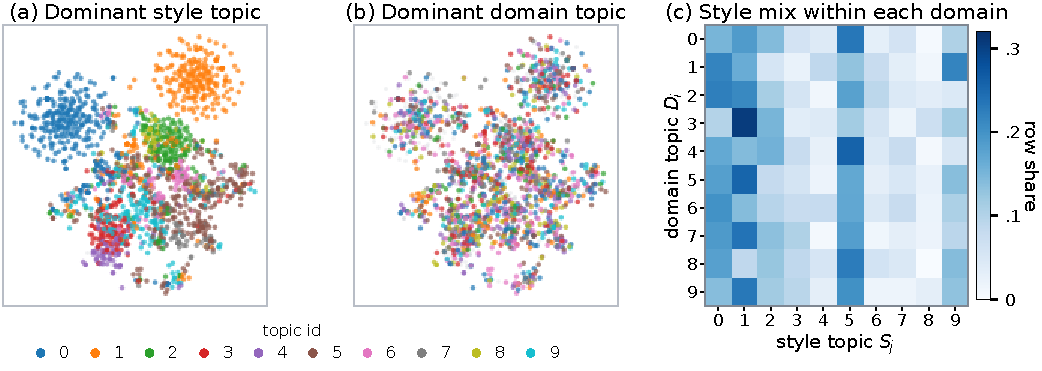
\includegraphics[width=\textwidth]{style_domain_comparison.pdf}
  \caption{One style-derived t-SNE slice colored by style (a) and domain (b), and the
  row-normalized domain--style table (c).  Gray means no retained topic.  Examples:
  $S_0$ \texttt{simp}, $S_1$ \texttt{rw}, $S_5$ \texttt{refine'/have}, $S_9$
  \texttt{apply/intro}; $D_1$ category theory, $D_2$ lists, $D_4$ measure theory, $D_8$ filters.}
  \label{fig:comparison}
\end{figure}

\paragraph{Measuring alignment.}
For the $n_c=1{,}628$ proofs assigned in both views, let $N_{ab}=|\{i:z_i^{(d)}=a,
z_i^{(s)}=b\}|$ count proofs in domain topic $a$ and style topic $b$.  Write
$p_{ab}=N_{ab}/n_c$, $p_{a+}=\sum_b p_{ab}$, and $p_{+b}=\sum_a p_{ab}$.  Mutual
information compares the joint table with the independent table:
\[
 I(D;S)=\sum_{a,b:p_{ab}>0}p_{ab}\log\frac{p_{ab}}{p_{a+}p_{+b}}.
\]
With $H(D)=-\sum_a p_{a+}\log p_{a+}$ and
$H(S)=-\sum_b p_{+b}\log p_{+b}$,
\[
 \operatorname{NMI}(D,S)=\frac{I(D;S)}{\sqrt{H(D)H(S)}}.
\]
Here $D$ and $S$ denote the random domain- and style-topic labels, and $H$ is Shannon entropy
(natural logarithms are used throughout).
Because a finite contingency table has positive mutual information even under random labels,
adjusted mutual information (AMI) subtracts its expected value under fixed marginals and scales
by the corresponding entropy ceiling.  AMI is therefore zero in expectation under the
permutation null and one for identical partitions.  Cram\'er's $V$ supplies a complementary
effect size based on squared cell deviations.  Neither statistic uses the plotted coordinates.

\paragraph{Different structures, weak correspondence.}
Panel (a)'s coordinates and colors both derive from style, so its coherence is expected.  The
evidence comes from domain colors on the unchanged coordinates and, independently of any
projection, the contingency table.

The style topics separate short normalization and rewriting proofs from longer structured
arguments: \texttt{simp} and \texttt{rw} proofs average 1.7 and 1.8 steps, while
\texttt{refine'/have} and \texttt{apply/intro} average 8.3 and 6.7.  Domain topics instead
recover category composition, lists, measure theory, polynomial algebra, filters, and integers.

Among the 1,628 proofs with nonzero assignments in both views, adjusted mutual information is
only $0.016$ (normalized mutual information $0.027$).  Let
$N_{a+}=\sum_bN_{ab}$ and $N_{+b}=\sum_aN_{ab}$ be the row and column totals.  Pearson's
chi-squared statistic $\chi^2$, its independence-model expected counts $E_{ab}$, and
Cram\'er's effect size $V$ are given below; the resulting $V=0.113$ is a small association:
\[
 \chi^2=\sum_{a,b}\frac{(N_{ab}-E_{ab})^2}{E_{ab}},\qquad
 E_{ab}=\frac{N_{a+}N_{+b}}{n_c},\qquad
 V=\sqrt{\frac{\chi^2}{n_c\min(K_s-1,K_d-1)}}=0.113,
\]
None of 20,000 permutations that preserve those totals produced so
large a statistic (Monte Carlo $p<5\times10^{-5}$), but the effect size says
\emph{detectable preference, not close alignment}.  No domain sends more than 30.5\% of its
proofs to one style; most maxima are 20--26\%.

\paragraph{Why this is interesting.}
Branches are usually related through shared objects and theorems.  This comparison points to a
second, procedural relation: subjects with disjoint vocabularies may reuse normalization,
extensionality, cases, construction, or rewriting, while neighboring subjects support different
styles.  A map based on proof-style distributions need not reproduce a premise graph; it could
identify methodological kinship---relation by how arguments are organized.

Subject is not irrelevant: Graph2Tac finds nearby concepts with similar proof structures
\cite{graph2tac}.  Our weak global association leaves room for such local conventions alongside
portable idioms.  This complements ML4PG's proof-pattern mining \cite{ml4pg,patterns} and
LeanDojo's separation of premise retrieval from tactic generation \cite{leandojo}.  SEPIA
models tactic sequences as inferred automata \cite{sepia}, while TacticToe learns which tactic
or mathematical technique suits a proof state from recorded human proofs \cite{tactictoe}; both
show why procedure is a meaningful object of study in its own right.

\paragraph{Limitations and next test.}
Proofs are short (median two tactics); annotations omit lemmas used internally by automation;
and labels reflect Lean/mathlib conventions.  A stronger test would embed state transitions,
compare full mixtures, and build branch networks from premises versus procedures.  Their
disagreement would test for methodological geometry distinct from dependency geometry.

This is a modest example of AI-assisted computational mathematics.  Proof assistants guarantee
local correctness; analysis asks global questions about practice.  AI makes those questions
cheaper to iterate, not to validate.  The prize is not an automated verdict, but a testable map
of formalized mathematical practice.

\vfill
\begin{thebibliography}{9}\footnotesize
\setlength{\itemsep}{0pt}
\bibitem{ml4pg} E. Komendantskaya, J. Heras, and G. Grov. ``Machine Learning in Proof General: Interfacing Interfaces.'' EPTCS 118, 2013.
\bibitem{patterns} J. Heras and E. Komendantskaya. ``Proof Pattern Search in Coq/SSReflect.'' arXiv:1402.0081, 2014.
\bibitem{leandojo} K. Yang et al. ``LeanDojo: Theorem Proving with Retrieval-Augmented Language Models.'' NeurIPS Datasets and Benchmarks, 2023.
\bibitem{graph2tac} L. Blaauwbroek et al. ``Graph2Tac: Online Representation Learning of Formal Math Concepts.'' arXiv:2401.02949, 2024.
\bibitem{sepia} T. Gransden, N. Walkinshaw, and R. Raman. ``SEPIA: Search for Proofs Using Inferred Automata.'' CADE-25, pp. 246--255, 2015.
\bibitem{tactictoe} T. Gauthier, C. Kaliszyk, J. Urban, R. Kumar, and M. Norrish. ``TacticToe: Learning to Prove with Tactics.'' Journal of Automated Reasoning 65(2), pp. 257--286, 2021.
\end{thebibliography}

\end{document}
